% Template for ICIP-2013 paper; to be used with:
%          spconf.sty  - ICASSP/ICIP LaTeX style file, and
%          IEEEbib.bst - IEEE bibliography style file.
% --------------------------------------------------------------------------
\documentclass{article}

%%%%%%%%%%%%%%%%%%%%%
% My usual settings %
%%%%%%%%%%%%%%%%%%%%%
\usepackage{JB_config_article}
\usepackage{spconf}

%%%%%%%%%%%%%%%%%%%%%%%%%%%
% Location of the figures %
%%%%%%%%%%%%%%%%%%%%%%%%%%%
\graphicspath{{Images/}} 

% % Example definitions.
% % --------------------
% \def\x{{\mathbf x}}
% \def\L{{\cal L}}

% Title.
% ------
\title{SCATTERING HIDDEN MARKOV TREE}
%
% Single address.
% ---------------
\name{J.B. REGLI, J. D. B. NELSON \thanks{Thanks DSTL/UCL Impact studentship for funding.}}
\address{UCL, Department of statistical science}
%
% For example:
% ------------
%\address{School\\
%	Department\\
%	Address}
%
% Two addresses (uncomment and modify for two-address case).
% ----------------------------------------------------------
%\twoauthors
%  {A. Author-one, B. Author-two\sthanks{Thanks to XYZ agency for funding.}}
%	{School A-B\\
%	Department A-B\\
%	Address A-B}
%  {C. Author-three, D. Author-four\sthanks{The fourth author performed the work
%	while at ...}}
%	{School C-D\\
%	Department C-D\\
%	Address C-D}
%
\begin{document}
%\ninept
%
\maketitle
%
\begin{abstract}
	A Scattering Convolutional Hidden Markov Tree (SCHMT) proposes a new inference mechanism for high-dimensional signals by combining the interesting signal representation created by the Scattering Transform (ST) to a powerful Probabilistic Graphical Model (PGM). \\
	A wavelet scattering network computes a signal translation invariant and  stable to deformations representation that still preserves the informative content of the signal. Such properties are acquired by cascading wavelet transform convolutions with nonlinear modulus and averaging operators.\\
	The network's structure and its distributions are described using a Hidden Markov Tree (HMT). This yield a generative model for high-dimensional inference. It offers a mean for performing several inference tasks among which are predictions. The scattering convolutional hidden Markov tree displays promising results on both classification and segmentation tasks of complex images.
\end{abstract}
%
\begin{keywords}
	Scattering network, Deep network, Hidden Markov Model, Classification
\end{keywords}
%
\section{Introduction}
\label{sec:Intro}

	The standard approach when working with high dimensional signals can be expressed as a two step procedure. First the data are projected in a feature space where the task at hand (classification, regression...) is simplified. Then prediction is done using a simple predictor in this new representational space. Predictors such as logistic regression or linear Support vector Machine are common choices. The mapping can either be hand-build ---\eg Fourier transform, wavelet transform--- or learned. In the last decade methods for learning the projection have drastically improved under the impulsion of the so called deep learning. Deep neural networks (sometime enriched by convolutional architecture) have been able to learn very effective representations for a given dataset and a given task. Such method have achieved state of the art on many standard problems as well as real world applications. And this despite using a very simple prediction mechanism ---on top of a very clever projection method.
		
	We proposes a method combining a recently proposed deterministic analytically tractable transformation inspired by deep convolutional to a probabilistic graphical model in order to create a powerful probabilistic tool to handle high dimensional prediction problems. In a similar fashion to the work done by Crouse on wavelet trees~\citep{crouse1998wavelet}, we propose to describe Mallat's scattering convolutional scattering transform~\citep{bruna2010classification} using a hidden Markov tree. Doing so we develop a new framework to model high-dimensional inputs. As opposed to the commonly used simple classification method, once trained our model can tackle prediction problems but also other inference tasks ---\eg generation, sensitivity analysis... %TODO: change to highlight low number of training example properties

	In  Section~\ref{sec:Background}  we  present  the  requisite  background  of high dimensional signal classification. Section~\ref{sec:SCN} introduces the Scattering Transform and some of its properties.   We  fuse these to an hidden Markov Tree concepts in Section~\ref{sec:SCHMT}, propose our Scattering Hidden Markov Tree (SCHMT), and describe the inferential machinery. In Section~\ref{sec:Experiments} we perform classification on a selection of standard datasets. We draw conclusions in Section~\ref{sec:Conclusion}
	
\section{Background}
	\label{sec:Background}

	
%TODO:
% DL --- pb: not analytically tractable & lot of training examples required
% ST --- pb: still require a few training examples
% WHMT --- pb: not powerfull enough


\section{Scattering networks}
\label{sec:SCN}
	
	A scattering network has the same general architecture as the Convolutional Neural Networks (CNNs) introduced by~\citet{lecun1995convolutional}. Both CNN and Scattering Convolutional Network (SCN) cascade a convolution step and a ``pooling'' non linearity. However while convolutional neural networks use kernel filters learned from the data with back-propagation algorithm, SCNs use a fixed wavelet filter bank~\cite{mallat}. The wavelet bank can then be designed to extract image features having the desired invariant~\cite{work translation invariant, work rotation invariant, work rigid motion}. 
	
	At each layer 
	
	
  \textbf{TBD} $\quad$ - $\quad$ 1 column and a half

  \begin{figure}[h]
    \begin{center}
      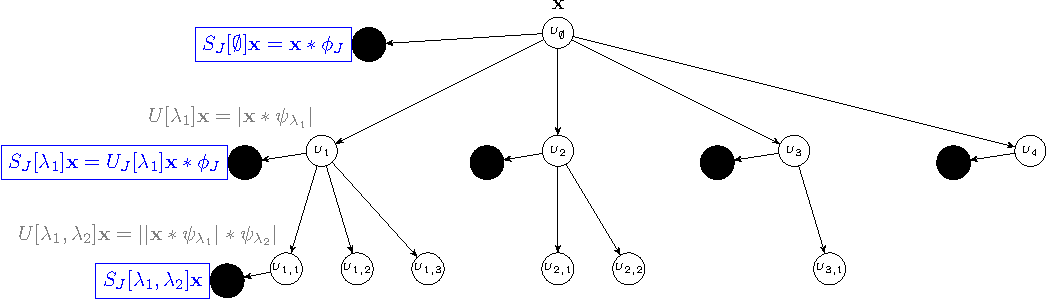
\includegraphics[width=3.3in, height=2in, keepaspectratio]{ST_freqDec_crop.pdf}
      \caption[Frequency decreasing scattering convolution network.]{\centering  Frequency decreasing scattering convolution network 	with $J=4$, $L=1$ and $M=2$. A node $i$ at scale $j_{i}$ generates $(j_{i}-1) \times L$ nodes. }
      \label{fig:SCN 2}
      % TODO: Narrow the gaps
    \end{center}	
  \end{figure}


% end of page 2

\section{The Scattering hidden Markov tree:}
\label{sec:SCHMT}

  \cite{Mallat ST} introduced the use of scattering networks combined with a support vector machine classifier to achieve competitive classification performance on some problems. However this method only provides a boolean label for each class. Some methods to express the output of an SVM as a probability exists~\cite{platt1999probabilistic} but they are just a rescaling of the output and not a true probabilistic approach. If one is interested in a true probabilistic model to describe the scattering coefficients, it is quite natural to try expressing them as a probabilistic graphical model. Furthermore generative models are known to be better for inference tasks when the number of training example is low~\cite{jordan2002discriminative}.\\
  
  \subsection{Hidden Markov tree model}
    \label{subsec:SCHMT/HMT model}
    %TODO Where to cite Crouse and Durand
    We propose an adaptation of those models to create a scattering convolutional hidden Markov tree composed of a set of visible nodes $\{\bfS_{i}\}_{i \in \mcalT}$ and a set of hidden node $\{\bfH_{i}\}_{i \in \mcalT}$. Both sets are organized in a tree structure such that for any index $i$ of the tree, $S_{i} \in \dsR$ and $H_{i} \in \llbracket 1,K \rrbracket$ where $K$ is the number of possible hidden states.
    The initial state is drawn from a discrete non uniform distribution $\pi_{0}$ such that, $\forall k \in \llbracket 1,K \rrbracket$ $\pi_{0}(k) = P(H_{0}=k)$.
    For any index $i$ of the tree, the emission distribution describes the probability of the visible node $S_{i}$ conditional to the hidden state $H_{i}$ such that, $\forall i \in \mcalT \, ,\, \forall k \in \llbracket1,K\rrbracket$ and $\forall s \in \dsR$ $P(S_{i}=s_{i}|H_{i}=k) = P_{\theta_{k,i}}(s)$, where $P_{\theta_{k,i}}$ belongs to a parametric distribution family and $\theta_{k,i}$ is the vector of emission parameters for the state $k$ and node $i$. In the remainder of the paper the emission distribution is Gaussian so that $P(S_{i}=s | H_{i}=k) = \mcalN(\mu_{k,i},\sigma_{k,i})$, where $\theta_{k,i}=(\mu_{k,i},\sigma_{k,i})$ with $\mu_{k,i}$ and $\sigma_{k,i}$ being respectively the mean and the variance of the Gaussian for the $k$-th value of the mixture and the node $i$.
    Finally the probability for the hidden node $H_{i}$ to be in a state $k$ given its father's state $g$ is characterized by a transition probability such that $\forall i \in \mcalT \backslash \{ 0 \} \; \forall g,k \in \llbracket1,K\rrbracket^{2}$ $\epsilon_{i}^{(gk)} = P(H_{i}= k | H_{\rho(i)}=g)$ where $\epsilon_{i}$ defines a transition probability matrix such that $P(H_{i}=k) = \sum_{g=1}^{K} \epsilon_{i}^{(gk)} P(H_{\rho(i)}=g)$.\\
    %TODO: find this formula in Durand article

    Such a model is pictured in Figure~\ref{fig:SCHMT 1} and for a given scattering architecture ---\ie fixed $M$, $J$ and $L$--- the SCHMT model is fully parametrized by,
    \begin{equation}
      \Theta = \big(\pi_{0}, \{ \epsilon_{i}, \{ \theta_{k,i} \}_{k\in\llbracket1,K\rrbracket} \}_{i\in\mcalT}\big).
      \label{eq:SCHMT - parameters}
    \end{equation}
    
    \begin{figure}[h]
      \begin{center}
				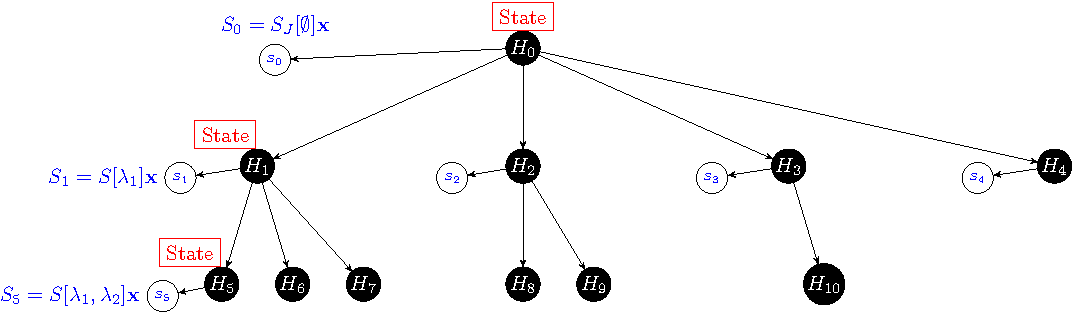
\includegraphics[width=3.3in, height=2in, keepaspectratio]{scat_HMT_crop.pdf}
				\caption{Scattering convolutional hidden Markov tree.}
				\label{fig:SCHMT 1}
				% TODO: Narrow the gaps
      \end{center}
    \end{figure}
    
    This model implies to do two assumptions on the scattering transform. First one need to assume --- $K$-populations--- that a signal’s scattering coefficients can be described by K clusters. This is a common assumptions for standard wavelets~\citep{kingsbury2001complex} and hence it can be extended to the scattering transform. The SCHMT also assumed ---persistence--- that the informative character of a coefficients is propagated across layers. This assumption is sound since ...
    %TODO K-pop and persistence

  \subsection{Learning the tree parameters}
    \label{subsec:SCHMT/Learning}    

    The SCHMT is trained using the smoothed version of the Expectation-Maximisation algorithm (\cite{someone}) for hidden Markov trees proposed by~\citep{Durand} and adapted to non-homogeneous and non-binary trees.
    
    \begin{center}
					\begin{algorithm}
						\textbf{Meta-parameters:}\\
							$K$\\
								
						\textbf{Initialization:}\\
							\tcp{$P_{\theta_{k,i}}(s_{i})$:}
							\For{All the nodes $i$ of the tree $\mcalT$}{
								$P_{\theta_{k,i}}(s_{i}) = \mcalN(s_{i} | \mu_{k,i},\sigma_{k,i})$
								}
								
							\tcp{Loop over the leaves $i$ of the tree:}
							\For{All the leaves $i$ of the tree $\mcalT$}{
								$\beta_{i}(k) = \frac{P_{\theta_{k,i}}(s_{i}) P(H_{i}=k)}{\sum_{g=1}^{K} P_{\theta_{g,i}}(s_{i}) P(H_{i}=g)}$\\
								$\beta_{i,\rho(i)}(k) = \sum_{g=1}^{K}\frac{\beta_{i}(g) \epsilon_{i}^{(kg)}}{P(H_{i}=g)} . P(H_{\rho(i)}=k)$ \\
								$l_{i} = 0$
								}
								
						\textbf{Induction:}\\
							\tcp{Bottom-Up loop over the nodes of the tree:}
							\For{All non-leaf nodes $i$ of the tree $\mcalT$}{
								$M_{i} = \sum_{k=1}^{K} P_{\theta_{k,i}}(s_{i}) \prod_{j \in c(i)} \frac{\beta_{j,i}(k)}{P(H_{i}=k)^{n_{i}-1}}$ \\
								$l_{i} = \log(M_{i}) + \sum_{j \in c(i)}l_{j}$\\
								$\beta_{i}(k) = \frac{P_{\theta_{k,i}(s_{i})} \prod_{j \in c(i)}(\beta_{j,i}(k))}{P(H_{i}=k) ^{n_{i}-1} M_{i}} $\\
								\For{All the children nodes $j$ of node $i$}{
									$\beta_{i\backslash c(i)}(k) = \frac{\beta_{i}(k)}{\beta_{i,j}(k)}$
									}
								$\beta_{i,\rho(i)}(k) = \sum_{g=1}^{K} \frac{\beta_{i}(g) \epsilon_{i}^{(kg)}}{P(H_{i}=g)} .P(H_{\rho(i)}=k)$
								}
						\caption{Smoothed upward algorithm.}
						\label{algo:Smoothed upward}		
					\end{algorithm}        
				\end{center}
    
				\begin{center}
					\begin{algorithm}
						\textbf{Meta-parameters:}\\
							$K$\\
								
						\textbf{Initialization:}\\
							$\alpha_{0}(k) = 1$
								
						\textbf{Induction:}\\
							\tcp{Top-Down loop over the nodes of the tree:}
							\For{All nodes $i$ of the tree $\mcalT\backslash\{0\}$}{
 								$\alpha_{i}(k) = \frac{1}{P(H_{i}=k)} \sum_{g=1}^{K} \alpha_{\rho(i)}(g) \epsilon_{i}^{(gk)} \beta_{\rho(i)\backslash i}(g) P(H_{\rho(i)}=g)$
								}
						\caption{Smoothed downward algorithm.}
						\label{algo:Smoothed downward}		
					\end{algorithm}        
				\end{center}
				
			\begin{center}
				\begin{algorithm}
					\textbf{Meta-parameters:}\\
						$K$,\\
						Distribution family for $P_{\theta}$ \tcp*{Here Gaussian}
						$N$ \tcp*{Number of observed realizations of the signal}
							
					\textbf{Initialization:}\\
						$\pi_{0}(k) = \frac{1}{N} \sum_{n=1}^{N} P(H_{0}^{n}=m|s_{0}^{n},\Theta^{l})$
							
					\textbf{Induction:}\\
						\tcp{Loop over the nodes of the tree:}
						\For{All nodes $i$ of the tree $\mcalT\backslash\{0\}$}{
							$P(H_{i}=k) = \frac{1}{N} \sum_{n=1}^{N} P(H_{i}^{n}=k|\bar{s}_{0}^{n},\Theta^{l})$,\\
							$\epsilon_{i}^{gk} = \frac{\sum_{n=1}^{N} P(H_{i}^{n} = k, H_{\rho(i)}^{n}=g |\bar{s}_{0}^{n}, \Theta^{l})} {N P(H_{\rho(i)}=k)}$,\\
							$\mu_{k,i} = \frac{\sum_{n=1}^{N} s_{i}^{n} P(H_{i}^{n} = k |\bar{s}_{0}^{n}, \Theta^{l})} {N P(H_{i}=k)}$,\\
							$\sigma_{k,i}^{2} = \frac{\sum_{n=1}^{N} (s_{i}^{n} - \mu_{k,i})^{2} P(H_{i}^{n} = k |\bar{s}_{0}^{n}, \Theta^{l})} {N P(H_{i}=k)}$.\\
							}
					\caption{M-step of the EM algorithm.}
					\label{algo:Mstep}
				\end{algorithm}        
			\end{center}
    
\section{Classification results}
	\label{sec:Experiments}


\section{Conclusion}
	\label{sec:Conlusion}




% Below is an example of how to insert images. Delete the ``\vspace'' line,
% uncomment the preceding line ``\centerline...'' and replace ``imageX.ps''
% with a suitable PostScript file name.
% -------------------------------------------------------------------------
% \begin{figure}[htb]
%   \begin{minipage}[b]{1.0\linewidth}
%     \centering
%     \centerline{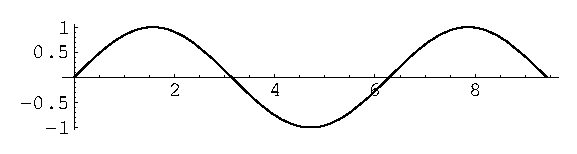
\includegraphics[width=8.5cm]{image1}}
% %   \vspace{2.0cm}
%     \centerline{(a) Result 1}\medskip
%   \end{minipage}
% %
%   \begin{minipage}[b]{.48\linewidth}
%     \centering
%     \centerline{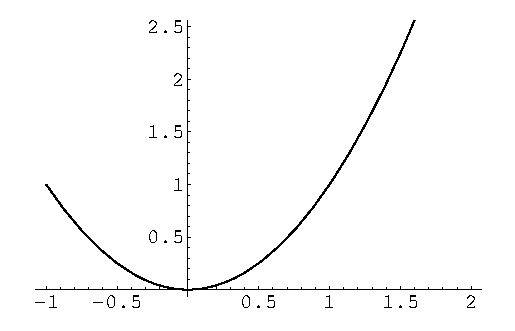
\includegraphics[width=4.0cm]{image3}}
% %   \vspace{1.5cm}
%     \centerline{(b) Results 3}\medskip
%   \end{minipage}
%   \hfill
%   \begin{minipage}[b]{0.48\linewidth}
%     \centering
%     \centerline{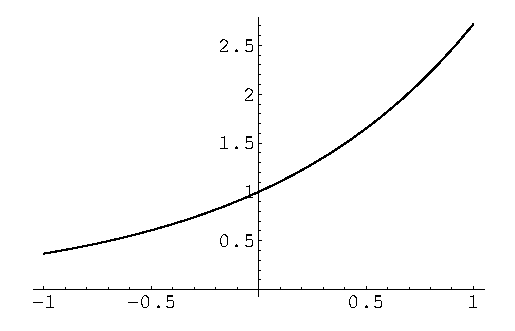
\includegraphics[width=4.0cm]{image4}}
% %   \vspace{1.5cm}
%     \centerline{(c) Result 4}\medskip
%   \end{minipage}
% %
%   \caption{Example of placing a figure with experimental results.}
%   \label{fig:res}
% \end{figure}


% To start a new column (but not a new page) and help balance the last-page
% column length use \vfill\pagebreak.
% -------------------------------------------------------------------------
\vfill
\pagebreak

\section{COPYRIGHT FORMS}
\l1abel{sec:copyright}

You must include your fully completed, signed IEEE copyright release form when
form when you submit your paper. We {\bf must} have this form before your paper
can be published in the proceedings.

\section{REFERENCES}
\label{sec:ref}
  


% References should be produced using the bibtex program from suitable
% BiBTeX files (here: strings, refs, manuals). The IEEEbib.bst bibliography
% style file from IEEE produces unsorted bibliography list.
% -------------------------------------------------------------------------
\bibliographystyle{IEEEbib}
%\bibliography{strings,refs}
% \bibliography{bib_icip}

\end{document}
